\documentclass[research]{BMSTU-IU8}

\usepackage{amssymb} % triangleeq
\usepackage{pdfpages}

\student{Железцов Н.В.}
\theme{
    Разработка методики и инструментов верификации \\
    соответствия TLA+ спецификации и исходного кода
}
\group{ИУ8-114}

\supervisor{Медведев Н.В.}
% \theme{Тест \hfill} % Тема для НИРСа заполняется по-другому
\studentFullName{Железцов Никита Владимирович}
\profile{20У474}
\speciality{10.05.01 <<Компьютерная безопасность>>}
\specialization{10.05.01\_01 <<Математические методы защиты информации>>}

\newacronym{ndjson}{NDJSON}{Newline Delimeted JSON.}
\newacronym{rm}{RM}{Resource Manager.}
\newacronym{tla}{TLA}{Temporal Logic of Actions.}
\newacronym{tm}{TM}{Transaction Manager.}
\newacronym{wal}{WAL}{Write-ahead log.}
\newacronym{json}{JSON}{JavaScript Object Notation.}



% \include{contents/terms}

\addbibresource{report.bib}

\begin{document}
    \maketitle % Титульный лист

    % 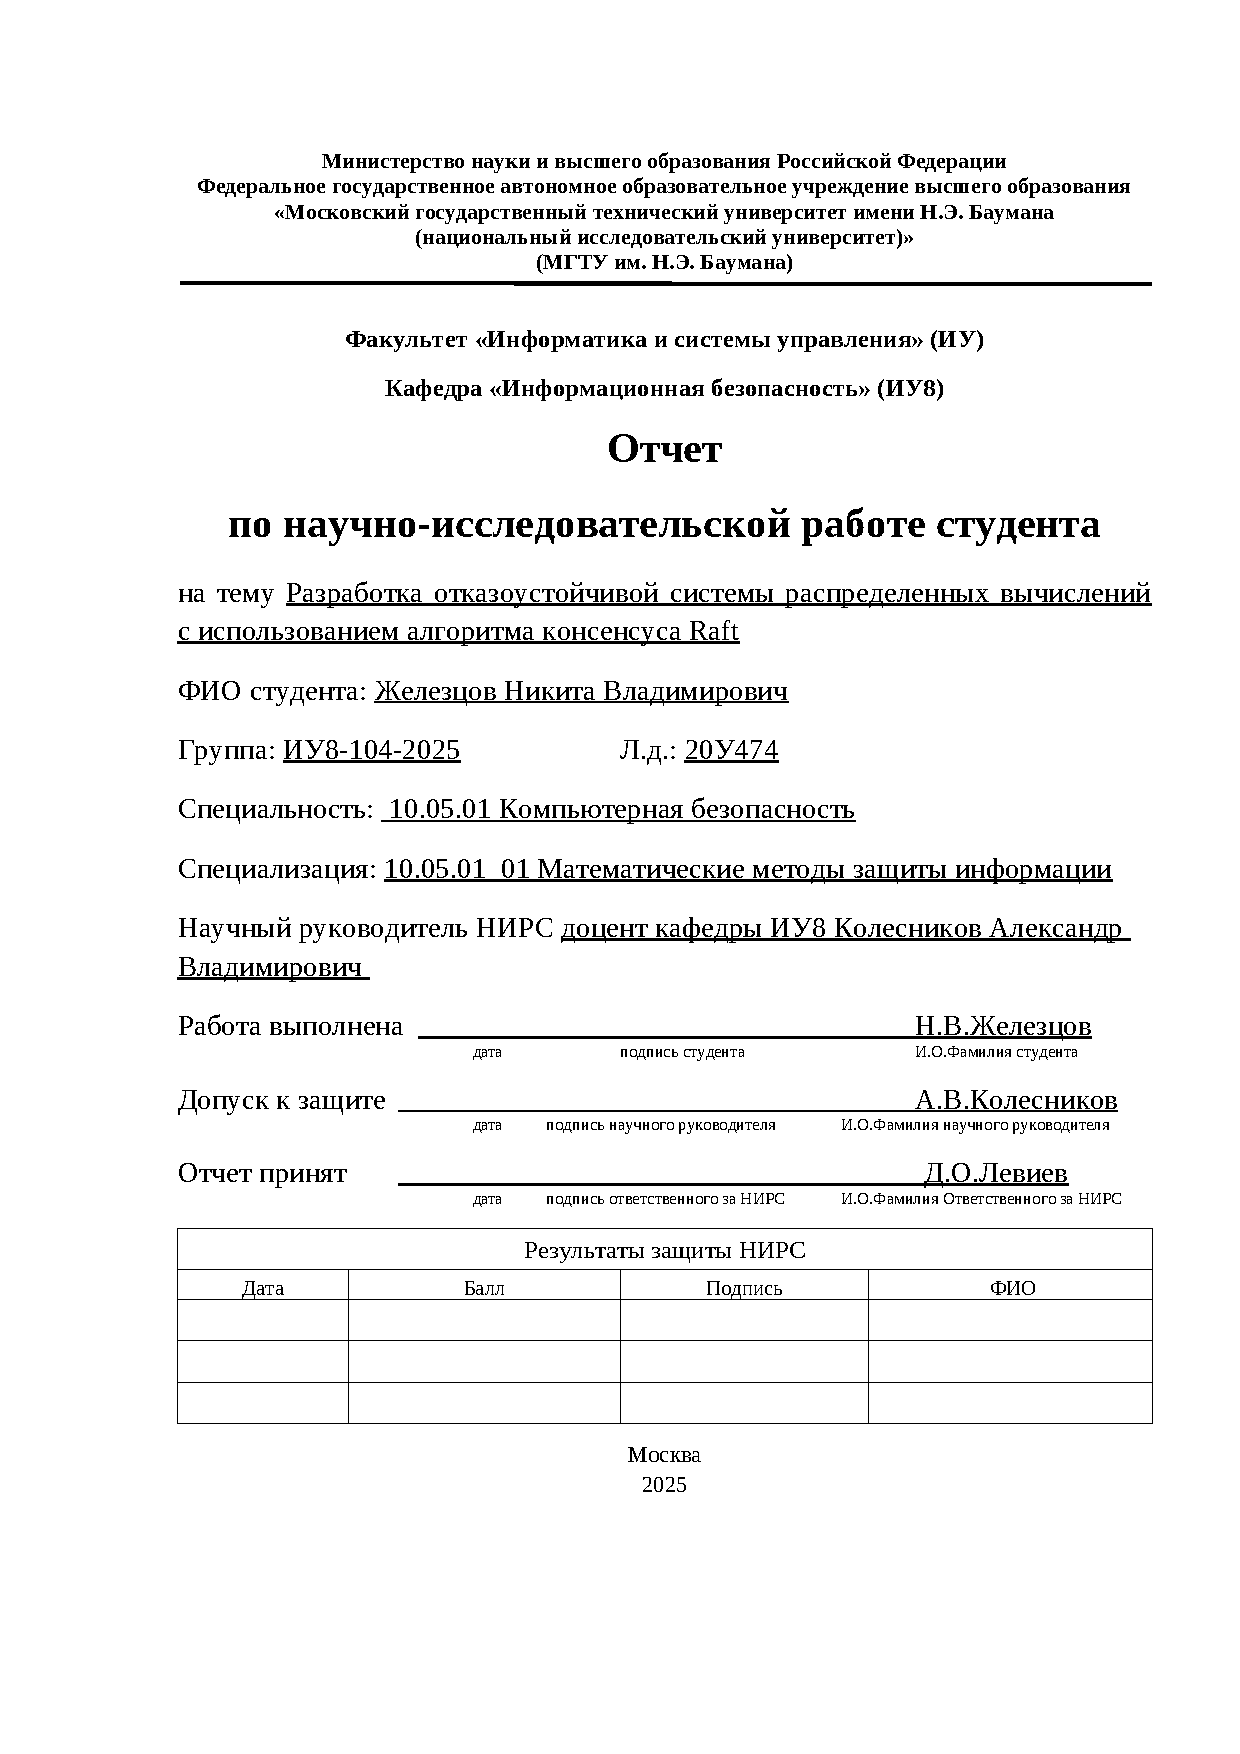
\includepdf[pages=-]{inc/titul-basic.pdf} % Задание
    \setcounter{page}{4} % Устанавливает счётчик страниц

    \abstract % Структурный элемент: РЕФЕРАТ

Ключевые слова: TLA+, трассировка, валидация трасс, модельная проверка,
распределённые системы, Two-Phase Commit.

Основная цель работы — разработка и апробация подхода к валидации
реализации распределённого алгоритма на основе формальной спецификации
TLA+ с использованием анализа трасс исполнения.

В работе рассматривается задача сопоставления поведения реальной
распределённой программы со спецификацией высокого уровня. В качестве
объекта исследования выбран алгоритм двухфазной транзакции (Two-Phase Commit),
широко применяемый для обеспечения согласованности в распределённых
транзакционных системах. Реализован прототип алгоритма на языке~C,
включающий координатора (Transaction Manager), участников (Resource
Managers) и сетевой сервер сообщений.

Для связывания кода со спецификацией разработан механизм инструментирования,
позволяющий фиксировать изменения только выбранных переменных спецификации,
а не полные состояния системы. Трассы исполнения формируются в формате
NDJSON и затем автоматически объединяются и подаются на вход модели
проверки TLC. Проверка корректности сводится к задаче ограниченной
модельной проверки, где TLC анализирует соответствие полученной трассы
спецификации TLA+.

В ходе экспериментов продемонстрировано обнаружение логической ошибки в
реализации алгоритма, связанной с некорректным учётом сообщений от участников.
Использование трассировки и формальной проверки позволило надёжно выявить
расхождение между спецификацией и реализацией в условиях недетерминированной
доставки сообщений.
 % Реферат

    \tableofcontents % Содержание
%    \termsanddefenitions % Термины и определения
    \listofabbreviations % Перечень сокращений и обозначений

    \introduction % Структурный элемент: ВВЕДЕНИЕ

Распределённые системы лежат в основе современных вычислительных платформ,
облачных сервисов и транзакционных приложений. Их корректность критически
важна, поскольку ошибки в алгоритмах координации, согласования и обмена
сообщениями могут приводить к потере данных, нарушению согласованности
состояния и отказам сервисов. При этом поведение распределённых систем
существенно усложняется из-за асинхронности, недетерминированности доставки
сообщений и возможных сбоев отдельных узлов.

Формальные методы позволяют повысить уверенность в корректности распределённых
алгоритмов за счёт построения строгих математических моделей. Одним из широко
применяемых инструментов является язык спецификаций TLA+
\cite{lamport2002specifying}, предназначенный для описания систем в терминах
состояний и переходов между ними. С помощью средства проверки моделей TLC
возможно исследование пространства состояний спецификации и доказательство
инвариантов.

Однако формальная верификация спецификации не гарантирует корректность
конкретной программной реализации алгоритма. На практике возникает разрыв между
абстрактной моделью и исполняемым кодом. В данной работе рассматривается подход
к сокращению этого разрыва путём сопоставления трасс исполнения реализации со
спецификацией TLA+.

\subsection*{Актуальность темы исследования}

Несмотря на широкое распространение формальных спецификаций в проектировании
распределённых алгоритмов, проблема согласованности спецификации и реализации
остаётся актуальной. Традиционные методы тестирования не обеспечивают полного
покрытия возможных сценариев взаимодействия компонентов, особенно в условиях
недетерминированного поведения сети.

Модельная проверка позволяет анализировать абстрактные модели, однако переход
от модели к реальному коду часто сопровождается упрощениями, оптимизациями или
изменением гранулярности атомарных действий. В результате возможны расхождения
между поведением реализации и предполагаемой спецификацией.

Перспективным направлением является модельная валидация исполнения (Model-Based
Trace Checking) \cite{howard2011tracechecking}, при которой реальные трассы
работы распределённой программы проверяются на соответствие формальной
спецификации с использованием средства модельной проверки. Такой подход
позволяет обнаруживать ошибки реализации, избыточные ограничения спецификации и
несоответствие уровня атомарности.

Разработка и практическая апробация метода валидации трасс исполнения по
спецификации TLA+ представляется актуальной задачей, направленной на повышение
надёжности распределённых систем. Этот метод активно применяется в индустрии
\cite{newcombe2015aws}.

\subsection*{Цель и задачи работы}

Целью данной научно-исследовательской работы является разработка метода
модельной валидации реализации распределённого алгоритма по формальной
спецификации TLA+ на основе анализа трасс исполнения.

Для достижения поставленной цели были сформулированы следующие задачи:

\begin{enumerate}
    \item Изучить теоретические основы языка спецификаций TLA+ и средства
модельной проверки TLC.
    \item Разработать механизм инструментирования реализации для регистрации
изменений переменных спецификации.
    \item Реализовать программный прототип распределённого алгоритма двухфазной
транзакции.
    \item Реализовать процедуру сопоставления трасс программы и спецификации
с использованием TLC.
    \item Провести экспериментальную валидацию и проанализировать полученные
результаты.
\end{enumerate}

Результатом работы является прототипный фреймворк, обеспечивающий сопоставление
трасс распределённой реализации с формальной спецификацией TLA+, а также
демонстрационная реализация алгоритма двухфазной транзакции, использованная для
апробации предложенного метода.
 % Введение
    \structure{ОСНОВНАЯ~ЧАСТЬ}

В основной части работы рассмотрены теоретические и практические аспекты
верификации алгоритмов методом модельной проверки трасс с использованием TLA+ и
TLC.

В разделе~1 изложены теоретические основы: описана модель вычислений в TLA+,
каноническая форма спецификаций, а также принцип проверки трасс исполнения
путём сопоставления их с поведениями формальной модели.

В разделе~2 представлена методика верификации. Формализована задача валидации
трасс. Описана реализация ограниченной спецификации (\texttt{TraceSpec}),
позволяющей свести задачу к ограниченной модельной проверке в TLC. Также
разработана библиотека инструментирования на языке C для автоматической
генерации трасс исполнения в формате NDJSON.

В разделе~3 методика продемонстрирована на примере алгоритма двухфазной
транзакции. Представлены реализация менеджера ресурсов и менеджера транзакций
на языке C, спецификация алгоритма на TLA+, а также процедура
инструментирования кода. Проведённая валидация позволила обнаружить логическую
ошибку в реализации, связанную с некорректной обработкой повторных сообщений
\texttt{Prepared}, что подтверждает практическую применимость предложенного
подхода.

\section{Теоретические основы}

В основе работы лежат методы формальной спецификации и модельной проверки
распределённых систем. Формальные методы позволяют описывать систему в виде
математической модели, задающей множество допустимых состояний и переходов
между ними, а также формулировать инварианты и свойства корректности. Однако
проверка спецификации не гарантирует корректность конкретной реализации. Для
сопоставления поведения программы с её формальной моделью используется
модельная валидация исполнения (Model-Based Trace Checking), позволяющая
проверять реальные трассы исполнения относительно формальной спецификации

\subsection{Формальная спецификация TLA+}

TLA+ — язык спецификаций, основанный на теории множеств, логике первого порядка
и темпоральной логике действий (англ. TLA, temporal logic of actions).

Темпоральная логика была введена Амиром Пнуэли в 1970-х годах \cite{amir70}.
Лесли Лэмпорт увидел недостаточность этой идеи для описания систем целиком и
пришёл к мысли о необходимости использовать конечные автоматы, которым
придавался смысл формул темпоральной логики, описывающих все возможные
пути исполнения. Таким образом родилась идея темпоральной логики действий
(TLA+), которая дополнила темпоральную логику следующим \cite{lamport08}:

\begin{itemize}
    \item инвариантность при повторении состояния;
    \item темпоральное использование кванторов существования;
    \item принятие в качестве атомарных формул не только предикатов состояния,
        но и формул действий.
\end{itemize}

TLA-спецификация — темпоральная формула, часто называемая $Spec$ и являющаяся
предикатом (утверждением) о поведении. Поведение представляет собой возможный
путь исполнения системы \cite{habrias06}.

Состоянием называется присваивание значений переменных, шагом называется пара
состояний. Теперь поведение можно представить как бесконечную последовательность
состояний, а шагами поведения можно назвать пару последовательных состояний
поведения. Предикатом состояния называется функция, результат которой —
логическое значение истина или ложь — соответствует утверждению о состоянии.
Действием называется функция, имеющая смысл предиката над шагом. В этой функции
участвуют как переменные первого шага, так и второго, которые обычно
отмечаются штрихом \cite{habrias06}.

$$
Spec \triangleq Init \wedge \Box [Next]_{(v_1, v_2, ..., v_n)}
$$

Здесь $Init$ — предикат состояния, $Next$ — действие, $v_i$ — переменные, $\Box$
— единственный в данной спецификации темпоральный оператор (истинно во всех
будущих состояниях).

TLC — это программа, которая по заданному TLA+ описанию системы и формулам
свойств перебирает состояния системы и определяет, удовлетворяет ли система
заданным свойствам.

Обычно работа с TLA+/TLC строится таким образом: описывается система в TLA+
(или уже реализованная, или та, которую собираются реализовать), формализуются
интересные свойства, запускается TLC для проверки этих свойств. Однако данная
работа ставит своей целью находить несоответствия работы программы и
спецификации, для чего и будет использоваться TLC.

\subsection{Модельная проверка трасс}

Одним из часто возникающих вопросов при использовании TLA+ является проверка
соответствия программной реализации формальной спецификации. В идеале хотелось
бы доказать, что реализация является уточнением высокоуровневой спецификации,
то есть что все возможные поведения программы допустимы спецификацией.
Однако на практике такой подход сталкивается с серьёзными проблемами
масштабируемости и применим лишь к очень небольшим программам.

Полная верификация (end-to-end verification) остаётся крайне дорогостоящей и
технически сложной задачей вне зависимости от используемых инструментов. Даже в
тех редких случаях, когда она осуществима, затраты времени и ресурсов делают её
непрактичной для большинства прикладных систем \cite{cirstea2024validating}.

Вместо этого в инженерной практике применяется более прагматичный подход —
\emph{model-based checking} или \emph{model-based trace-checking}
\cite{howard2011tracechecking}. Его идея заключается не в доказательстве того,
что \emph{все} возможные поведения реализации соответствуют спецификации, а в
проверке того, что \emph{наблюдаемые} поведения ей соответствуют.

Подход состоит из следующих этапов:

\begin{enumerate}
    \item Реализация инструментируется таким образом, чтобы фиксировать
    существенные события и изменения состояний.
    \item Во время выполнения системы формируется трасса исполнения.
    \item Полученная трасса интерпретируется как ограничение на поведение
    формальной спецификации.
    \item Средство модельной проверки (в данном случае TLC) проверяет,
    существует ли поведение спецификации, согласованное с данной трассой.
\end{enumerate}

Таким образом, задача сводится к проверке воспроизводимости наблюдаемой
последовательности переходов в рамках формальной модели.

В отличие от классической модельной проверки, здесь не требуется перебирать всё
пространство состояний системы. Проверяется лишь конкретная трасса, что
существенно снижает вычислительную сложность. При этом метод применим к
распределённым системам, где трассы могут собираться с нескольких узлов и
агрегироваться для последующего анализа.

Данный подход имеет ряд преимуществ:

\begin{itemize}
    \item низкая стоимость интеграции в существующий процесс разработки;
    \item возможность использования стандартных средств модельной проверки;
    \item обнаружение некорректных переходов даже при отсутствии
    явных сбоев выполнения;
    \item применимость к системам, написанным на различных языках
    программирования.
\end{itemize}

Следует отметить, что метод не является строгой формальной гарантией
корректности, поскольку анализируется лишь конечное множество наблюдаемых
трасс. Однако при достаточном объёме тестовых запусков вероятность обнаружения
ошибок существенно возрастает. Как показывает практика применения формальных
методов в индустрии \cite{howard2024ccf}, даже
частичная формальная проверка позволяет обнаруживать серьёзные ошибки на ранних
этапах разработки.

    \section{Методика верификации}

Предлагаемая методика верификации основана на сопоставлении трасс исполнения
распределённой реализации с формальной спецификацией, написанной на языке TLA+.
Общая схема подхода представлена на рисунке~\ref{fig:arch}.

\begin{figure}
  \centering
  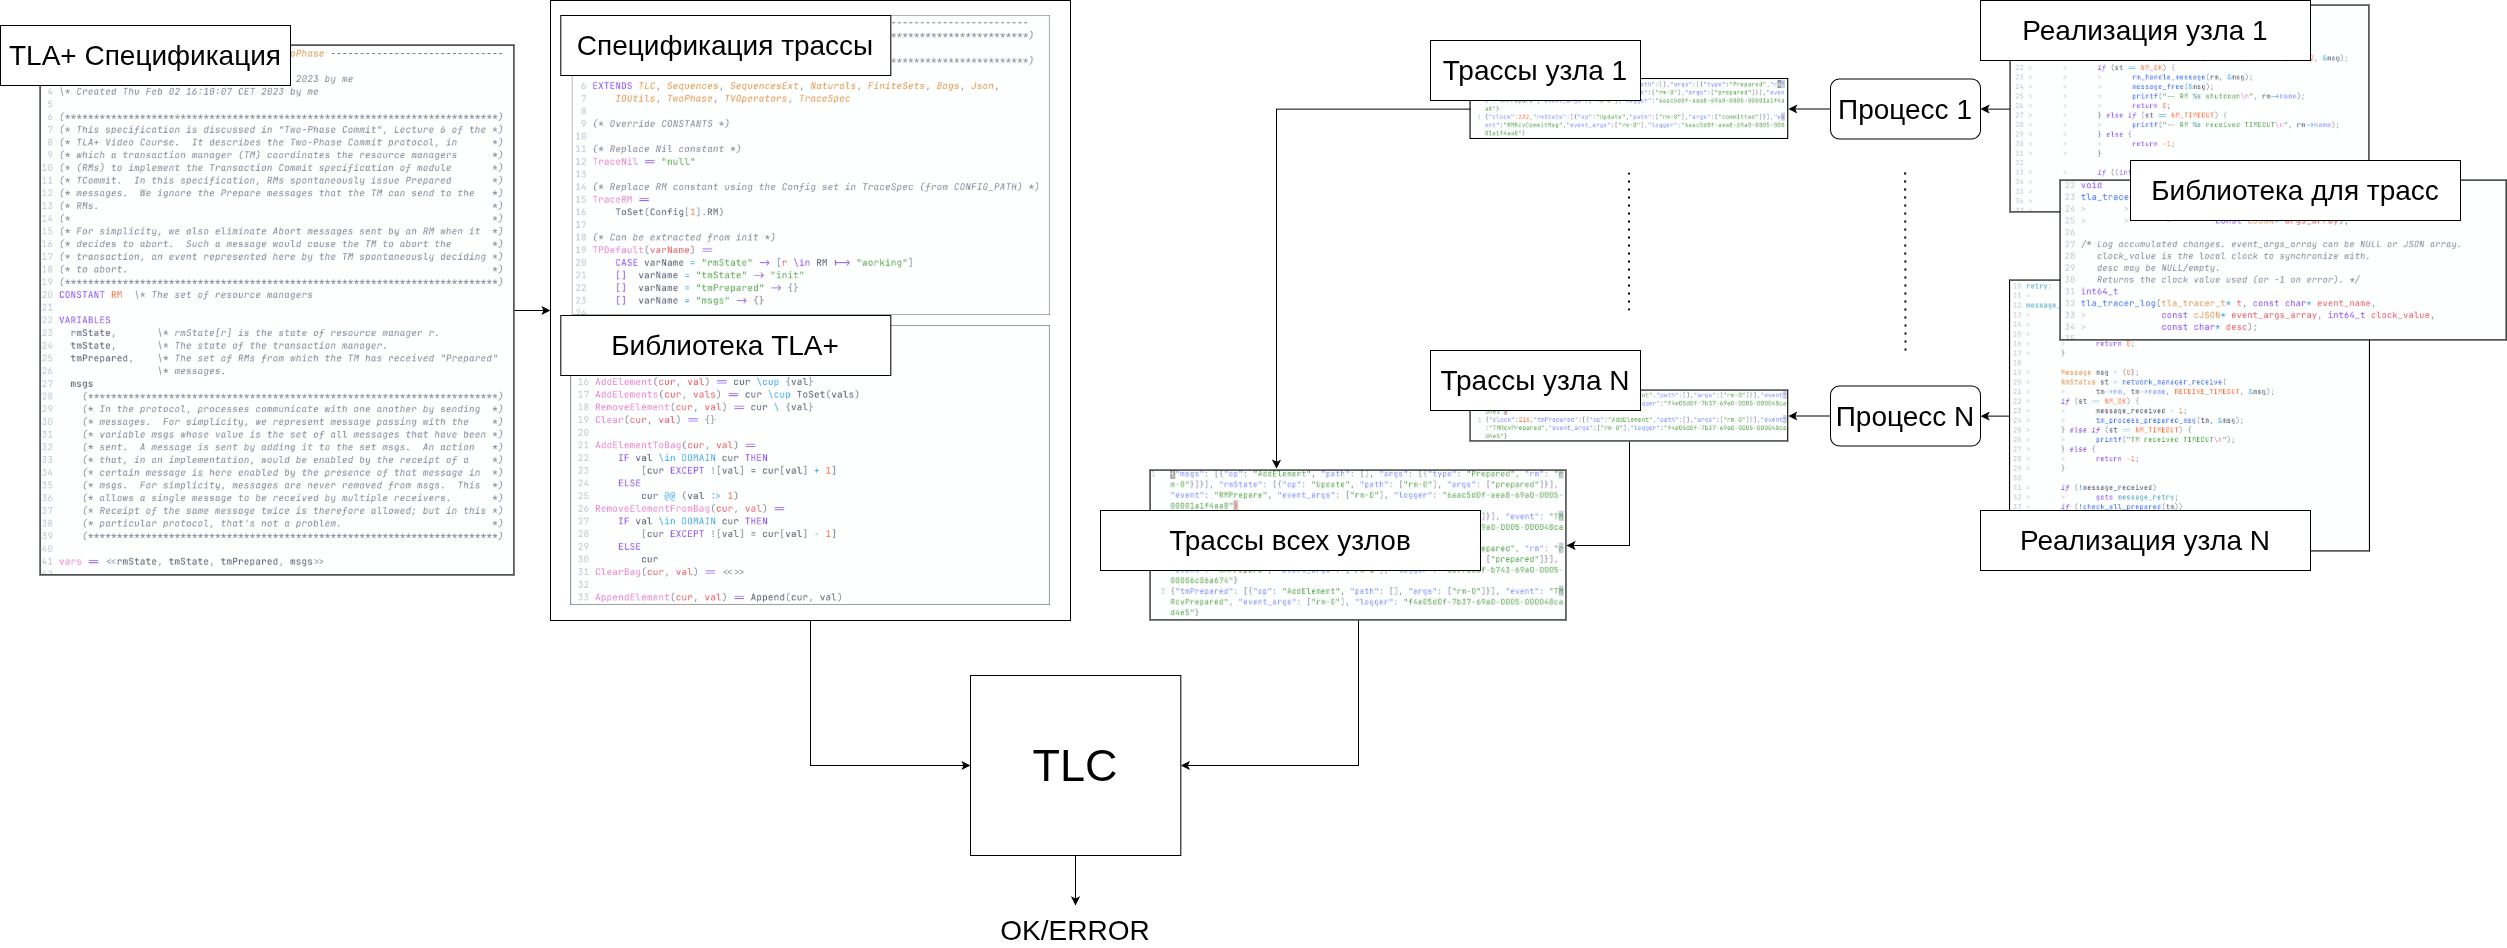
\includegraphics[scale=0.17]{inc/arch.png}
  \caption{Методика верификации}
  \label{fig:arch}
\end{figure}

Исходными артефактами являются:

\begin{itemize}
    \item программная реализация алгоритма.
    \item формальная спецификация этого алгоритма на языке TLA+.
\end{itemize}

Спецификация задаёт множество допустимых состояний системы и переходов между
ними, однако не содержит сведений о конкретной реализации. Реализация, в свою
очередь, выполняется в распределённой среде, где возможны различные порядки
доставки сообщений и недетерминированные сценарии выполнения.

Для сопоставления поведения реализации со спецификацией используется
инструментирование кода. В реализацию внедряется библиотека трассировки,
которая фиксирует события, соответствующие переходам спецификации, а также
изменения переменных спецификации. При выполнении системы каждый процесс
(координатор и участники) формирует собственную трассу в формате JSON,
содержащую последовательность операций обновления логических переменных модели.

Полученные локальные трассы агрегируются в единый глобальный файл, отражающий
наблюдаемую последовательность изменений состояния всей распределённой системы.
Таким образом, формируется абстрактное представление исполнения, выраженное в
терминах переменных TLA+, а не в терминах низкоуровневых операций кода.

Для проверки корректности трассы используется дополнительная спецификация
(Trace Specification), построенная на основе исходной TLA+ спецификации. Она
расширяет её таким образом, чтобы поведение модели было ограничено наблюдаемой
последовательностью изменений. Иными словами, трасса интерпретируется как
частичное ограничение на допустимые переходы модели.

Далее средство модельной проверки TLC используется для проверки существования
поведения спецификации, согласованного с данной трассой. Если TLC подтверждает
корректность, это означает, что наблюдаемое исполнение допустимо спецификацией.
В противном случае обнаруживается расхождение между реализацией и моделью, и
TLC предоставляет контрпример, позволяющий локализовать проблему.

\subsection{Задача валидации трасс}

Задача валидации трасс формулируется следующим образом. Пусть $S$ ---
множество конечных поведений, удовлетворяющих спецификации $Spec$, и пусть
$T$ --- множество конечных поведений, представляемых трассой исполнения,
где переменным, значения которых не были зафиксированы в трассе,
разрешается принимать произвольные значения. Трасса считается совместимой
со спецификацией тогда и только тогда, когда
\[
S \cap T \neq \varnothing.
\]
Иными словами, существует хотя бы одно поведение спецификации,
согласующееся с наблюдаемой трассой. Заметим, что мы не проверяем условие
уточнения (refinement) высокоуровневой спецификации трассой, выражаемое
как $T \subseteq S$. Такое условие было бы слишком строгим в случае,
когда значения некоторых переменных не фиксируются в трассе и могут
выбираться недетерминированно.

Рис~\ref{fig:traces-search} иллюстрирует идею. Слева изображается линейная
цепочка состояний, соответствующая трассе, полученной из инструментированной
реализации. Справа --- граф состояний, определяемый спецификацией TLA+.
Требуется проверить, существует ли в графе состояний спецификации путь, который
можно сопоставить данной трассе.

\begin{figure}
  \centering
  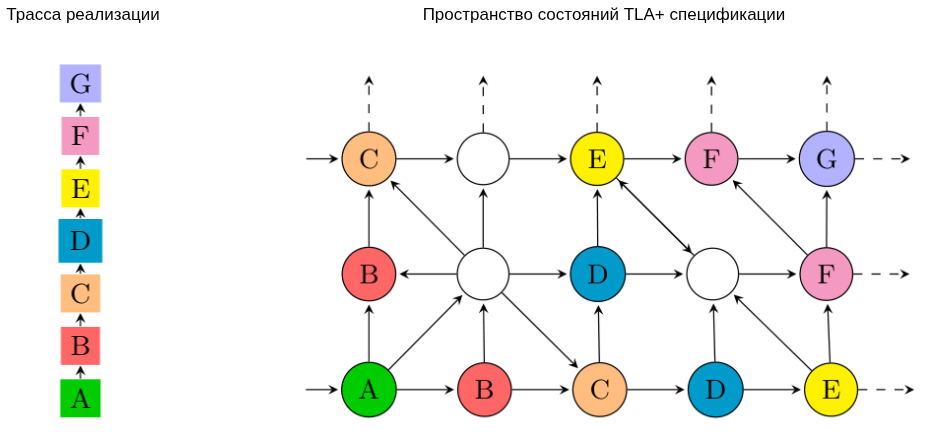
\includegraphics[scale=0.5]{inc/traces-search.png}
  \caption{Валидация трассы как поиск пути в пространстве состояний}
  \label{fig:traces-search}
\end{figure}

Первое состояние трассы должно соответствовать некоторому начальному состоянию
спецификации. Далее для каждого последующего шага трассы необходимо найти хотя
бы одного преемника уже сопоставленного состояния, который соответствует
следующему элементу трассы. Из-за неполной информации о значениях переменных
одному шагу трассы может соответствовать несколько состояний спецификации. Если
для некоторого состояния спецификации не существует допустимого продолжения,
согласующегося со следующим элементом трассы, такая ветвь поиска отбрасывается.
Трасса признаётся совместимой, если существует по крайней мере один путь в
графе состояний спецификации, который полностью соответствует всей
последовательности шагов трассы.

Следует учитывать дополнительную тонкость: атомарные шаги реализации не обязаны
в точности совпадать с атомарными переходами спецификации. Один шаг программы
может соответствовать нескольким шагам TLA+ или, наоборот, некоторым переходам
спецификации может не соответствовать явного события в трассе. Поэтому задача
валидации сводится к проверке существования пути в пространстве состояний
спецификации при дополнительных ограничениях, задаваемых трассой. Практически
эта редукция реализуется с помощью модельного проверяющего TLC.

В общем случае разработчик должен явно задать соответствие между
именами событий в трассе и действиями спецификации, а также между
именами логируемых переменных и переменными TLA+.

\subsection{Реализация инструментирования спецификации}

Множество $S$ конечных поведений, удовлетворяющих исходной спецификации,
задаётся формулой TLA+ $Spec$. Для того чтобы охарактеризовать пересечение $S
\cap T$, то есть поведения спецификации, совместимые с трассой исполнения, к
спецификации добавляются дополнительные ограничения. Таким образом, задача
сводится к построению ограниченной спецификации, учитывающей информацию из
трассы.

В разработанном фреймворке для этого используется отдельный модуль
\texttt{TraceSpec}, предоставляющий операторы для построения ограниченной
версии исходной спецификации. Его часть приведена на
рис.~\ref{fig:trace-spec-1}.

\begin{figure}
  \centering
  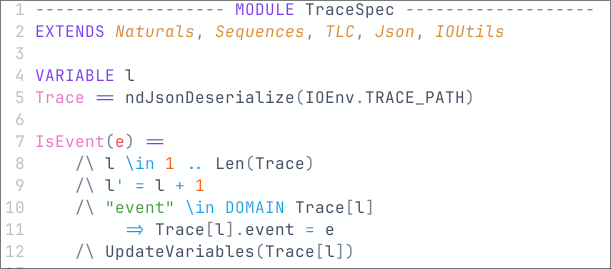
\includegraphics[scale=0.5]{inc/trace-spec-1.png}
  \caption{Реализация $IsEvent()$ из модуля $TraceSpec$}
  \label{fig:trace-spec-1}
\end{figure}

Модуль объявляет переменную $l$, обозначающую номер текущей строки трассы.
Оператор $Trace$ десериализует NDJSON-файл и представляет трассу программы в
виде последовательности записей, каждая из которых соответствует одной записи
журнала исполнения.

Оператор $IsEvent(e)$ инкапсулирует обработку текущей строки трассы.
Он проверяет, что индекс $l$ корректен, увеличивает его на единицу и,
если в записи явно указано поле \texttt{"event"}, проверяет соответствие
ожидаемому имени действия. Параметры события, если они заданы, учитываются
далее. Кроме того, вызывается оператор $UpdateVariables$ (см.
рис~\ref{fig:trace-spec-2}, который накладывает ограничения на значения
переменных спецификации.

\begin{figure}
  \centering
  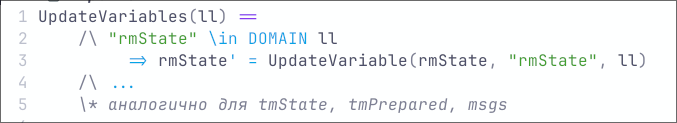
\includegraphics[scale=0.5]{inc/trace-spec-2.png}
  \caption{Реализация $UpdateVariables()$}
  \label{fig:trace-spec-2}
\end{figure}

Данный оператор проверяет, присутствует ли в текущей строке трассы обновление
соответствующей переменной. Если да, новое значение вычисляется с помощью
вспомогательного оператора $UpdateVariable$ (также определенного в
\texttt{TraceSpec}), который принимает старое значение переменной и описание
операции из JSON-записи.

Для каждого действия исходной спецификации строится соответствующее
действие ограниченной спецификации, получаемое конъюнкцией с
предикатом $IsEvent$. Пример приведен на рис.~\ref{fig:trace-spec-3}

\begin{figure}
  \centering
  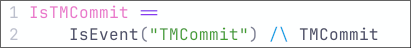
\includegraphics[scale=0.5]{inc/trace-spec-3.png}
  \caption{Пример действия ограниченной спецификации}
  \label{fig:trace-spec-3}
\end{figure}

Поскольку TLC вычисляет формулы слева направо, сначала применяются ограничения
из трассы (обновляются переменные), после чего проверяется, удовлетворяет ли
полученное состояние предикату действия исходной спецификации. Для переменных,
значения которых не зафиксированы в трассе, TLC может недетерминированно
выбирать подходящие значения.

Для параметризованных действий учитываются аргументы, указанные в трассе.
Например:

Таким образом, если в трассе указан конкретный параметр, рассматривается
соответствующий экземпляр действия; иначе TLC разрешается выбрать любой
допустимый параметр.

Общее отношение перехода ограниченной спецификации $TraceNext$ определяется как
дизъюнкция всех таких ограниченных действий. Построение этой спецификации в
большинстве случаев является систематическим и может быть автоматизировано.

При проверке TLC вычисляет все возможные преемники текущего состояния. Даже
если из некоторого состояния нельзя продолжить сопоставление с трассой, в
пространстве состояний могут существовать другие ветви, соответствующие трассе.
Поэтому не следует включать проверку deadlock для ограниченной спецификации.

Для валидации трасс использовать постусловие, приведенное на
рис.~\ref{fig:trace-spec-4}.

\begin{figure}
  \centering
  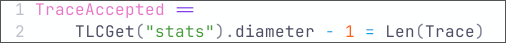
\includegraphics[scale=0.5]{inc/trace-spec-4.png}
  \caption{Условие валидации соответствия трасс}
  \label{fig:trace-spec-4}
\end{figure}

Если данное условие выполняется, существует поведение спецификации, полностью
соответствующее трассе. Если нет, пересечение $S \cap T$ пусто, и трасса
несовместима со спецификацией. В этом случае TLC не может предоставить единый
контрпример (поскольку подходящего поведения не существует), однако может
вывести максимальный префикс поведения спецификации, совпадающий с трассой.

Следует отметить, что при неполной трассировке возможны ложноположительные
результаты: если трасса содержит слишком мало информации (например, фиксирует
только длину исполнения без обновлений переменных и имён действий), модельный
проверяющий может недетерминированно подобрать значения переменных так, что
будет найдено совместимое поведение. Поэтому степень детализации трассировки
напрямую влияет на точность валидации и размер пространства поиска.

\subsection{Библиотека инструментирования реализации}

Для сопоставления поведения реализации с формальной спецификацией TLA+ была
разработана библиотека инструментирования на языке~C \cite{tlacimpl}. Её задача
--- фиксировать изменения логических переменных модели и формировать трассу
исполнения в формате NDJSON, пригодную для последующей валидации средствами
TLC.

Библиотека реализует следующий принцип:

\begin{enumerate}
    \item Во время выполнения программы фиксируются изменения логических
    переменных спецификации через \texttt{notify\_change}.
    \item В точке линейризации вызывается \texttt{log}, формируя
    атомарную запись трассы.
    \item Полученный NDJSON-файл представляет последовательность
    логических шагов, которые могут быть сопоставлены с действиями
    TLA+ спецификации.
    \item Полученные от разных процессов трассы можно объединить, используя
Python скрипт \texttt{trace\_merger.py}.
\end{enumerate}

Библиотека предоставляет абстракцию \texttt{tla\_tracer\_t}, инкапсулирующую
логику накопления изменений переменных и формирования записей трассы. Основной
интерфейс представлен функциями, приведенными на рис~\ref{fig:tlac-impl}.

\begin{figure}
  \centering
  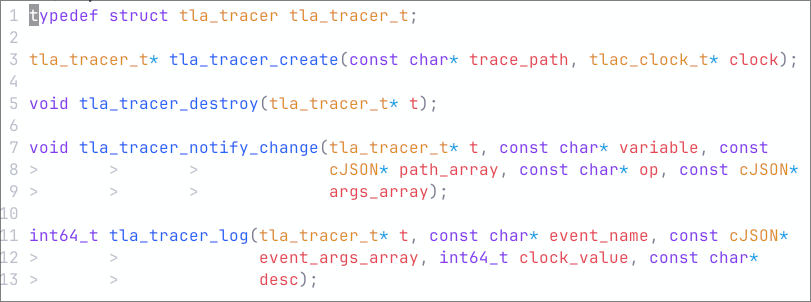
\includegraphics[scale=0.5]{inc/tlac-impl.png}
  \caption{Интерфейс библиотеки инструментирования реализации}
  \label{fig:tlac-impl}
\end{figure}

Для согласования порядка событий используется абстракция часов (см.
\texttt{tlac\_clock\_t} в функции \texttt{tla\_tracer\_create}). Часы могут
быть:
\begin{itemize}
    \item локальными (в памяти процесса),
    \item файловыми (для процессов на одном компьютере),
\end{itemize}

Все трассировщики синхронизируются через один и тот же механизм часов,
что обеспечивает монотонность временных меток как внутри одного процесса,
так и глобально между несколькими процессами. Возвращаемое функцией
\texttt{tla\_tracer\_log} значение --- это использованная временная метка.

Функция \texttt{tla\_tracer\_log} создаёт одну запись в файле трассы.
В запись включаются (см. рис~\ref{fig:json}):

\begin{itemize}
    \item временная метка (\texttt{"clock"});
    \item все изменения переменных, накопленные после предыдущего вызова
\texttt{log};
    \item имя события (\texttt{"event"});
    \item аргументы события (\texttt{"event\_args"}, например, ID узла).
\end{itemize}

После записи буфер изменений очищается. Таким образом, один вызов \texttt{log}
соответствует одному логическому шагу спецификации, объединяя несколько
изменений переменных в атомарную запись трассы.

В реализации допускается логирование только подмножества переменных
спецификации. В этом случае модельный проверяющий будет восстанавливать
отсутствующую информацию недетерминированным образом. Тем не менее, более
подробная трассировка (фиксация и переменных, и параметров действий)
существенно сокращает пространство поиска TLC и повышает достоверность
результатов валидации.

\begin{figure}
  \centering
  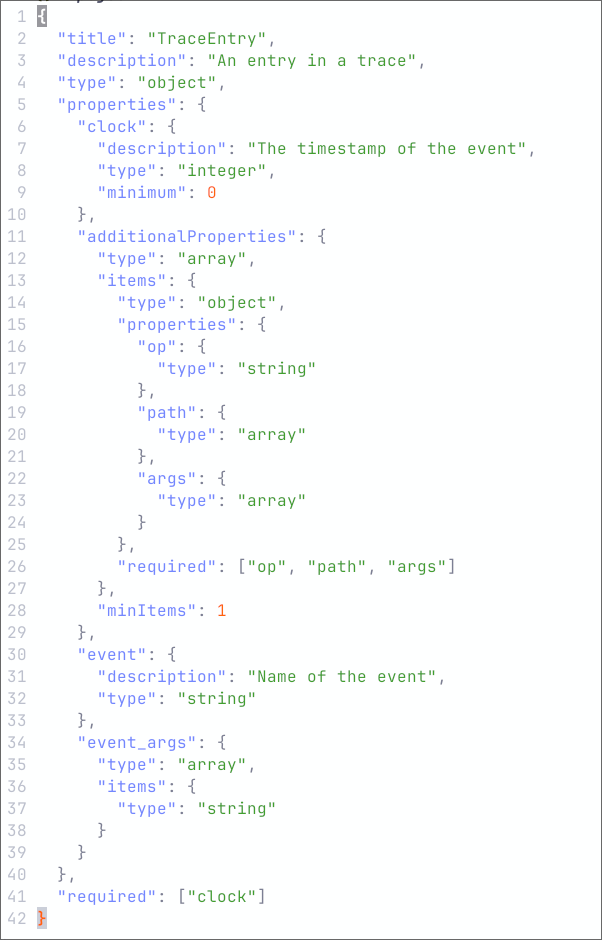
\includegraphics[scale=0.5]{inc/json.png}
  \caption{JSON структура записи трассы}
  \label{fig:json}
\end{figure}

    \section{Демонстрационный пример: алгоритм двухфазной транзакции}

Протокол двухфазной транзакции (Two-Phase Commit, 2PC) представляет собой
распределённый алгоритм атомарного подтверждения, предназначенный для
координации нескольких процессов, участвующих в одной распределённой
транзакции. Его задача заключается в том, чтобы все участники либо
зафиксировали изменения (commit), либо откатили их (abort), обеспечивая
тем самым атомарность выполнения.

Протокол использует выделенный процесс-координатор (Transaction Manager, TM)
и множество участников (Resource Managers, RM). Координатор принимает
окончательное решение о результате транзакции, а участники выполняют
локальные действия и голосуют за подтверждение или отмену.

Работа протокола основана на следующих предположениях:

\begin{itemize}
    \item у каждого узла имеется стабильное хранилище (WAL);
    \item узлы могут аварийно завершаться, но не выходят из строя навсегда;
    \item записи журнала не теряются и не повреждаются при сбое;
    \item любые два узла могут обмениваться сообщениями.
\end{itemize}

В отсутствие отказов выполнение транзакции состоит из двух фаз, оно
представлено на рисунке~\ref{fig:twopc}.

\begin{figure}
  \centering
  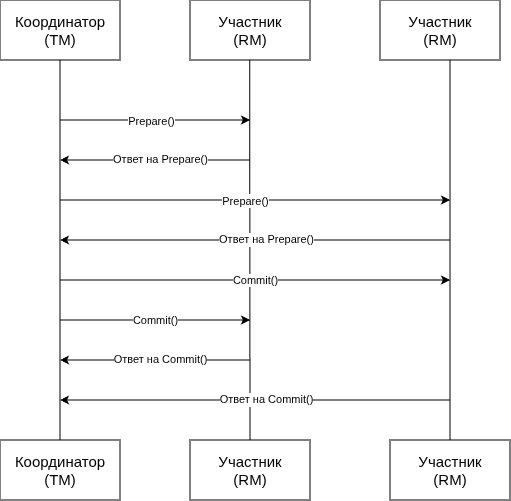
\includegraphics[scale=0.5]{inc/twopc.png}
  \caption{Двухфазный комммит}
  \label{fig:twopc}
\end{figure}

1. Фаза запроса подтверждения (voting phase).

\begin{enumerate}
    \item Координатор отправляет всем участникам сообщение
    \texttt{Prepare} (запрос на подтверждение).
    \item Каждый участник выполняет локальную часть транзакции до точки
    фиксации.
    \item Участник записывает соответствующие записи в журнал (undo/redo).
    \item Участник отправляет координатору голос:
    \begin{itemize}
        \item \texttt{Yes} (готов зафиксировать), если локальная часть
        выполнена успешно;
        \item \texttt{No} (отказ), если обнаружена ошибка.
    \end{itemize}
\end{enumerate}

2. Фаза завершения (commit phase).

\begin{itemize}
    \item Если координатор получил голос \texttt{Yes} от всех участников,
    он принимает решение \texttt{Commit}.
    \item В противном случае принимается решение \texttt{Abort}.
\end{itemize}

После принятия решения:

\begin{enumerate}
    \item Координатор рассылает сообщение \texttt{Commit} или \texttt{Abort}
    всем участникам.
    \item Каждый участник выполняет соответствующее действие:
    фиксирует изменения или откатывает их.
    \item Участник освобождает ресурсы и отправляет подтверждение
    (ACK) координатору.
    \item После получения всех подтверждений координатор завершает транзакцию.
\end{enumerate}

Протокол обеспечивает атомарность: либо все участники фиксируют изменения,
либо ни один из них не фиксирует. Однако 2PC является \emph{блокирующим}
протоколом. Если координатор выходит из строя после получения голосов
\texttt{Yes}, участники, отправившие согласие, вынуждены ожидать решения,
не имея возможности самостоятельно завершить транзакцию.

Кроме того, одновременный отказ координатора и одного из участников в фазе
завершения может привести к неопределённости состояния до восстановления
узлов. Несмотря на эти ограничения, протокол двухфазной транзакции широко
используется благодаря своей простоте и строгой атомарной семантике
\cite{bernstein2009ptp}.

\subsection{Реализация алгоритма на С}

В рамках работы был реализован прототип распределённого алгоритма
двухфазной транзакции на языке~C. Реализация состоит из двух типов
процессов: менеджер транзакции (Transaction Manager, TM) и набор
менеджеров ресурсов (Resource Manager, RM). Обмен сообщениями между
процессами вынесен в отдельный компонент сетевого взаимодействия
(\texttt{NetworkManager}) и происходит через центральный сервер сообщений (см.
\texttt{server.c} в реализации \cite{twophaseimpl}), который принимает команды
отправки и выборки сообщений и хранит их в буфере.

Логика протокола соответствует высокоуровневой модели: каждый RM выполняет
локальную работу, затем сообщает TM о готовности, а TM собирает готовности
от всех RM и после этого принимает решение о завершении транзакции
(в демонстрационном варианте --- всегда \texttt{Commit}, а \texttt{Abort} возможен
по таймауту).

\subsubsection{Менеджер ресурсов}

Основной цикл RM реализован в функции \texttt{rm\_run} (фрагмент кода приведён
на рис~\ref{fig:rm-impl}).

\begin{figure}
  \centering
  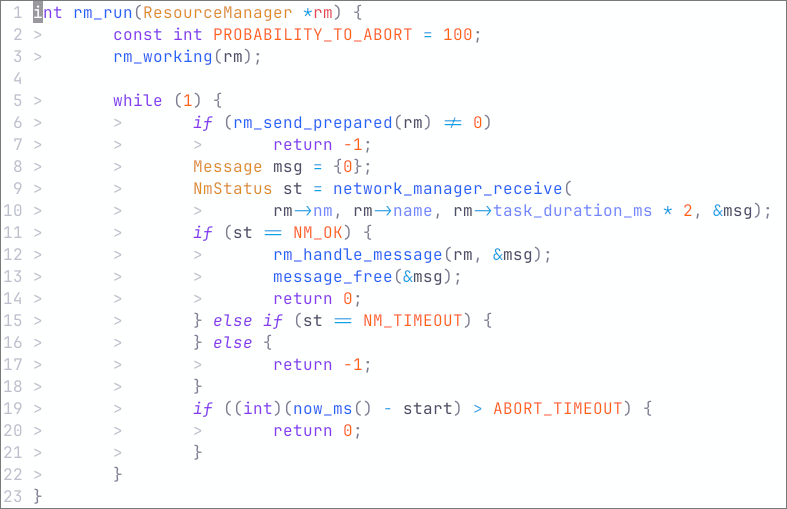
\includegraphics[scale=0.5]{inc/rm-impl.png}
  \caption{Реализация менеджера ресурсов}
  \label{fig:rm-impl}
\end{figure}

После старта процесс моделирует выполнение локальной операции
(\texttt{rm\_working}), затем переходит в фазу ожидания решения TM. Ключевой
элемент протокола --- повторная отправка сообщения о готовности при
отсутствии ответа от TM: если по истечении таймаута ответа нет, RM повторяет
отправку \texttt{Prepared}. Эта деталь важна, потому что в реальных
распределённых системах сообщения могут теряться или задерживаться, и
участникам необходимо обеспечивать прогресс протокола повторными попытками.

В реализации повторная отправка реализуется естественным образом за счёт цикла
\texttt{while (1)}: на каждой итерации RM отправляет \texttt{Prepared}, затем
вызывает \texttt{network\_manager\_receive} с конечным таймаутом. Если
результат --- \texttt{NM\_OK}, значит TM прислал решение (\texttt{Commit} или
\texttt{Abort}), и RM завершает работу после обработки сообщения. Если
результат --- \texttt{NM\_TIMEOUT}, RM не меняет состояние и переходит к
следующей итерации, тем самым повторяя отправку готовности.

Дополнительно предусмотрено аварийное завершение по общему дедлайну
(\texttt{ABORT\_TIMEOUT}): если RM слишком долго не получает решения, он
прекращает работу (в прототипе это моделирует сбой или невозможность завершить
транзакцию).

Важно отметить, что функция \texttt{rm\_send\_prepared} обновляет локальное
состояние RM: первый раз при отправке \texttt{Prepared} RM переходит в
состояние ``prepared'' и фиксирует соответствующее событие. Повторные отправки
\texttt{Prepared} не меняют состояние RM, но создают ситуации, в которых TM
может получить дубликаты сообщений.

\subsubsection{Менеджер транзакций}

Менеджер транзакций реализован в функции \texttt{tm\_run} (приведена на
рис~\ref{fig:tm-impl}). TM хранит список управляемых RM (\texttt{rm\_names}) и
множество RM, от которых уже получено \texttt{Prepared} (\texttt{prepared}).
После запуска предусмотрена инициализационная задержка
\texttt{init\_duration\_ms} --- она позволяет дать RM время отправить первые
сообщения \texttt{Prepared} прежде, чем TM начнёт интенсивно опрашивать сеть.
Эта задержка удобна для экспериментов и повторяемости, хотя не является
обязательной частью самого протокола.

\begin{figure}
  \centering
  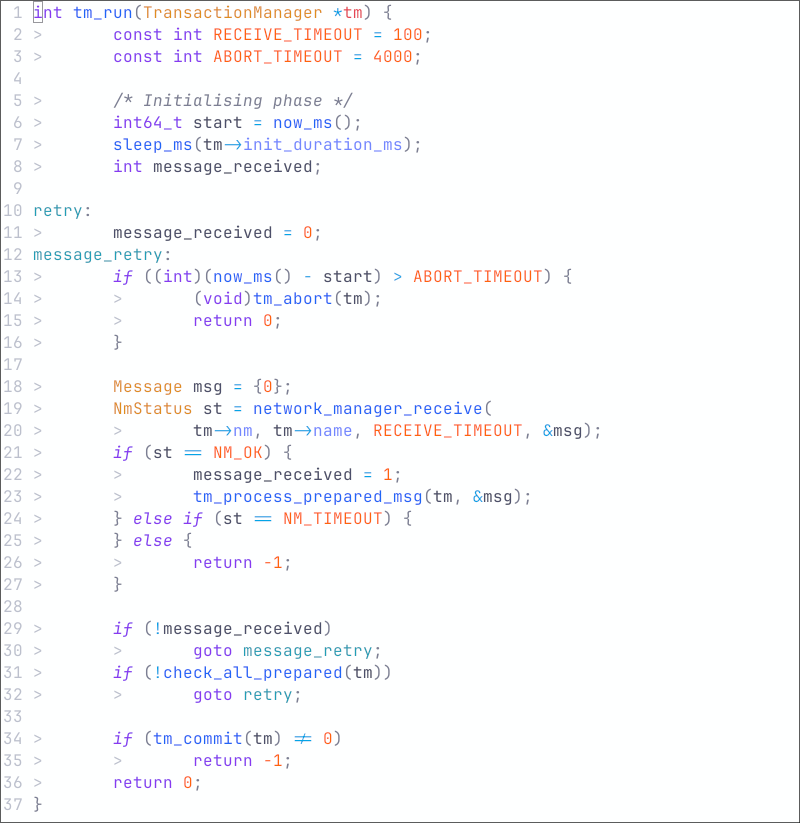
\includegraphics[scale=0.5]{inc/tm-impl.png}
  \caption{Реализация менеджера транзакций}
  \label{fig:tm-impl}
\end{figure}

Далее TM входит в цикл ожидания сообщений. Получение сообщений осуществляется
вызовом \texttt{network\_manager\_receive} с таймаутом
\texttt{RECEIVE\_TIMEOUT}. Если сообщение получено и оно содержит
\texttt{Prepared}, TM добавляет отправителя в структуру \texttt{prepared}.
После каждой успешно обработанной доставки проверяется условие завершения
подготовительной фазы: \texttt{check\_all\_prepared}. Если условие истинно, TM
рассылает всем RM сообщение \texttt{Commit} и завершает работу.

Если же сообщений долго нет и превышен общий дедлайн \texttt{ABORT\_TIMEOUT},
TM выбирает условие \texttt{Abort} и уведомляет всех участников об отмене
транзакции.

\subsection{Спецификация алгоритма на TLA+}

В качестве формальной модели используется спецификация алгоритма двухфазной
транзакции (Two-Phase Commit) на языке TLA+. Данная спецификация основана на
публичном примере из репозитория TLA+ Examples \cite{tlaexamplestwopc} и
приведена в сокращенном виде на рис.~\ref{fig:twopc-tla}.

\begin{figure}
  \centering
  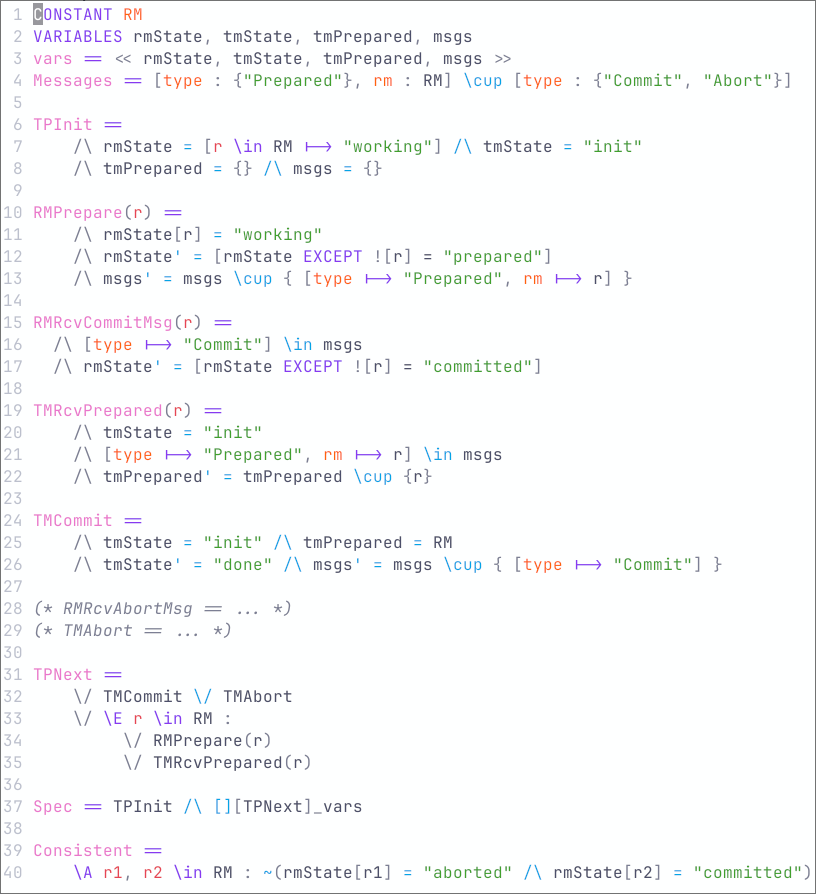
\includegraphics[scale=0.5]{inc/twopc-tla.png}
  \caption{Спецификация алгоритма двухфазной транзакции}
  \label{fig:twopc-tla}
\end{figure}

Спецификация описывает взаимодействие менеджера транзакции (TM) и множества
менеджеров ресурсов (RM), которые должны согласованно принять решение о
фиксации (commit) или откате (abort) транзакции. Менеджеры ресурсов отправляют
сообщения о готовности выполнить транзакцию, а менеджер транзакции, получив
голоса всех участников, принимает итоговое решение и рассылает соответствующее
сообщение.

Модуль сначала объявляет константу \texttt{RM}, представляющую множество
идентификаторов менеджеров ресурсов, и четыре переменные состояния:

\begin{itemize}
    \item \texttt{rmState} --- функция, отображающая каждый RM в его
    локальное управляющее состояние;
    \item \texttt{tmState} --- состояние менеджера транзакции;
    \item \texttt{tmPrepared} --- множество RM, объявивших готовность;
    \item \texttt{msgs} --- множество сообщений, отправленных в системе.
\end{itemize}

Начальное состояние задаётся предикатом \texttt{TPInit}: все RM находятся
в состоянии \texttt{"working"}, TM --- в состоянии \texttt{"init"},
а множества \texttt{tmPrepared} и \texttt{msgs} пусты.

Далее определяются действия, описывающие переходы системы.
Например, действие \texttt{RMPrepare(r)} моделирует объявление RM
с идентификатором \texttt{r} своей готовности: его состояние
изменяется на \texttt{"prepared"}, а в множество сообщений добавляется
соответствующее сообщение.

Действие \texttt{TPNext} задаёт отношение перехода системы как дизъюнкцию
всех возможных действий. Формула \texttt{Spec} объединяет начальное
условие и отношение перехода, задавая полную спецификацию поведения.

Свойства спецификации могут проверяться средствами TLC и TLAPS.
В частности, инвариант \texttt{Consistent} утверждает, что не существует
двух RM, один из которых завершил транзакцию успешно, а другой --- отменил.

Затем с помощью модуля \texttt{TraceSpec} была разработана специализированная
обёртка над спецификацией алгоритма двухфазной транзакции — модуль
\texttt{TwoPhaseTrace}. Его задача заключается в связывании конкретной
спецификации \texttt{TwoPhase} с механизмом обработки трасс: поведение
спецификации ограничивается конкретной последовательностью событий, полученной
из исполнения программы. Ее сокращенная версия представлена на
рис.~\ref{fig:twopc-spec}.

\begin{figure}
  \centering
  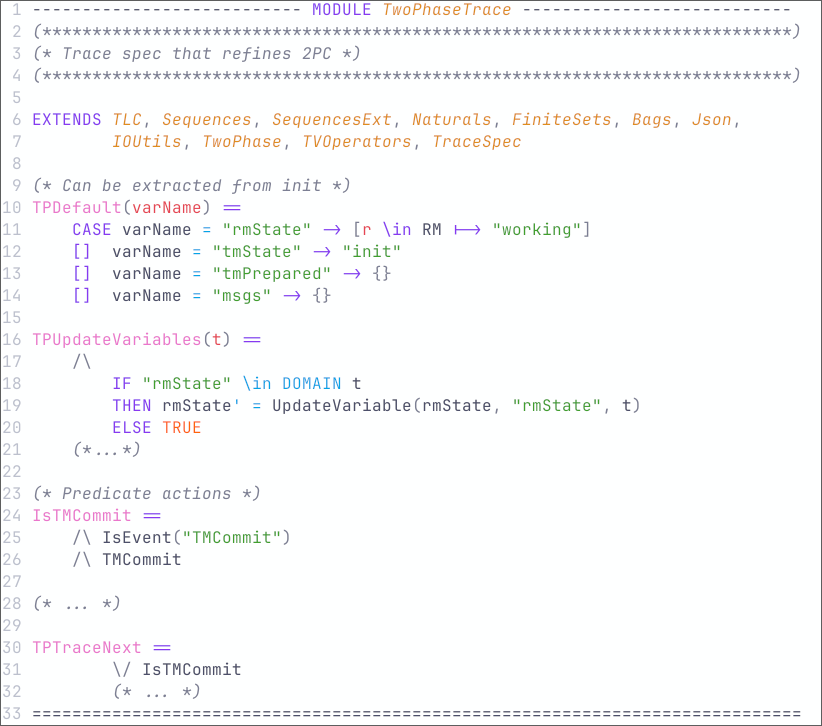
\includegraphics[scale=0.5]{inc/twopc-spec.png}
  \caption{Обертка над спецификацией алгоритма для верификации трасс}
  \label{fig:twopc-spec}
\end{figure}

\subsection{Инструментирование реализации}

После разработки реализации и спецификации алгоритма двухфазной транзакции
следующим шагом стало инструментирование этой реализации. Цель
инструментирования --- установить явное соответствие между действиями кода на
языке~C и переходами TLA+ спецификации (\texttt{RMPrepare},
\texttt{TMRcvPrepared}, \texttt{TMCommit}, \texttt{RMRcvCommitMsg} и др.).

Инструментирование выполнялось в \emph{точках линеаризации} --- местах,
где реализация завершает логически атомарный шаг протокола и обновляет
разделяемое состояние (например, изменение локального состояния RM или
добавление сообщения в множество \texttt{msgs}). В этих точках:

\begin{enumerate}
    \item регистрируются изменения переменных спецификации через
    \texttt{notify\_change};
    \item выполняется вызов \texttt{tracer\_log}, связывающий накопленные
    изменения с конкретным действием TLA+.
\end{enumerate}

\begin{figure}
  \centering
  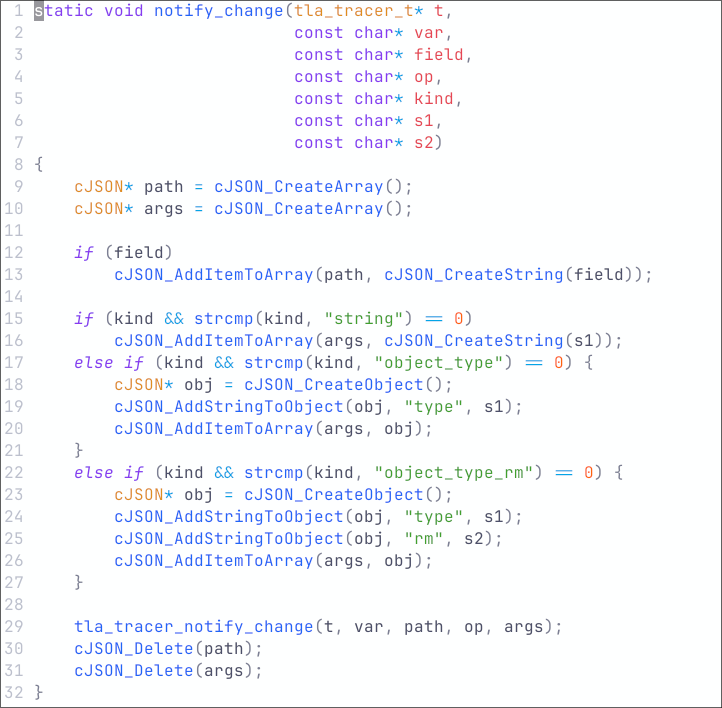
\includegraphics[scale=0.4]{inc/notify-change-impl.png}
  \caption{Вспомогательная функция для инструментирования алгоритма}
  \label{fig:notify-change}
\end{figure}

Для удобства использования библиотеки была реализована вспомогательная функция
\texttt{notify\_change}, упрощающая формирование JSON-структур \texttt{path} и
\texttt{args}. На рис~\ref{fig:notify-change} приведена сокращённая версия
функции, отражающая её логическую структуру:

Рассмотрим инструментирование отправки сообщения \texttt{Prepared}
менеджером ресурсов. В реализации эта логика сосредоточена в функции
\texttt{rm\_send\_prepared}, которая приведена на рис~\ref{fig:rm-tlac-impl}

\begin{figure}
  \centering
  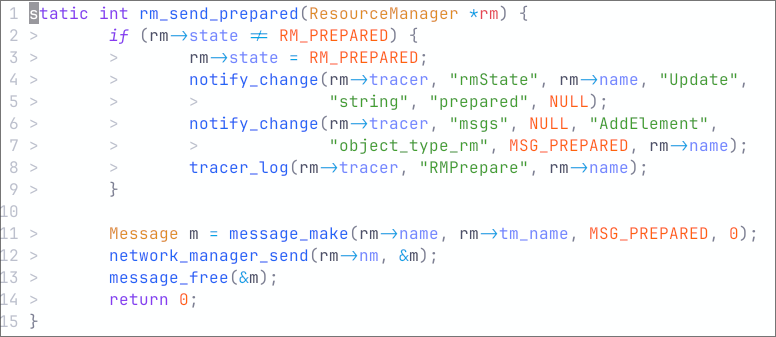
\includegraphics[scale=0.5]{inc/rm-tlac-impl.png}
  \caption{Реализация отправки сообщения prepared}
  \label{fig:rm-tlac-impl}
\end{figure}

Для RM с именем \texttt{"rm-0"} соответствующая запись трассы имеет вид,
приведенный на рис.~\ref{fig:rm-json}

\begin{figure}
  \centering
  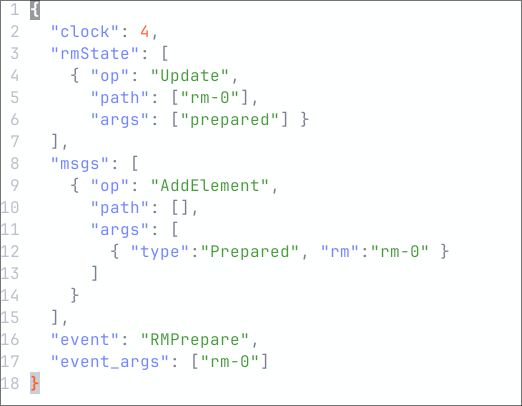
\includegraphics[scale=0.5]{inc/rm-json.png}
  \caption{Полученное сообщение трассы}
  \label{fig:rm-json}
\end{figure}

\subsection{Проверка соответствия TLA+ спецификации и исходного кода}

В процессе сопоставления реализации алгоритма двухфазной транзакции со
спецификацией на TLA+ был выявлен дефект в реализации, связанный с обработкой
сообщений \texttt{Prepared} менеджером транзакции (TM).

В корректной реализации TM должен фиксировать множество
менеджеров ресурсов, от которых получены сообщения \texttt{Prepared},
и принимать решение о фиксации транзакции только тогда, когда
\[
tmPrepared = RM,
\]
то есть когда каждый участник проголосовал за выполнение транзакции.

Однако возможна упрощённая реализация, в которой вместо множества хранится лишь
счётчик полученных сообщений \texttt{Prepared}. В этом случае условие
готовности проверяется сравнением счётчика с числом менеджеров ресурсов. Такая
реализация работает корректно, если сообщения не теряются и не дублируются.

Тем не менее, в нашей системе RM при истечении таймаута повторно отправляет
сообщение \texttt{Prepared}. Если TM не проверяет уникальность отправителя,
повторное сообщение от одного и того же RM может быть учтено несколько раз. Это
приводит к преждевременной фиксации, когда ещё не все участники объявили
готовность.

Дефект был выявлен при первом запуске \texttt{run\_pipeline\_until\_fail.sh}. В
журнале исполнения видно, что RM~\texttt{rm-0} несколько раз отправляет
сообщение \texttt{Prepared} из-за тайм-аута (см. рис.~\ref{fig:test-1}).

\begin{figure}
  \centering
  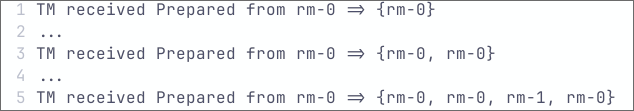
\includegraphics[scale=0.5]{inc/test-1.png}
  \caption{Повторное получение сообщения от rm-0}
  \label{fig:test-1}
\end{figure}

В результате TM принимает решение \texttt{Commit}, несмотря на то что
RM~\texttt{rm-3} ещё не отправил сообщение о готовности. Это видно из трассы:
событие \texttt{TMCommit} происходит до того, как TM получит \texttt{Prepared}
от \texttt{rm-3}. Фрагмент NDJSON-трассы приведен на рис.~\ref{fig:test-2}.

\begin{figure}
  \centering
  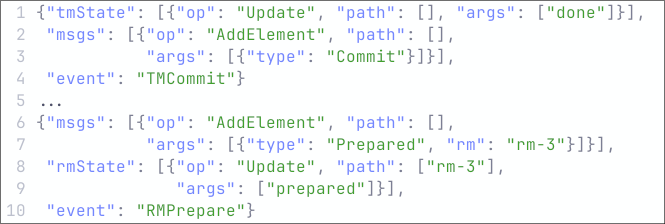
\includegraphics[scale=0.5]{inc/test-2.png}
  \caption{Часть трассы, иллюстрирующая некорректное поведение TM}
  \label{fig:test-2}
\end{figure}

То есть подтверждение транзакции произошло до получения готовности от всех RM,
что противоречит предикату \texttt{TMCommit} в спецификации.

При проверке трассы TLC ограниченная спецификация \texttt{TwoPhaseTrace} не
смогла сопоставить событие \texttt{TMCommit} с допустимым переходом исходной
модели.  Это означает, что в пространстве состояний спецификации не существует
поведения, в котором переход \texttt{TMCommit} возможен при текущем значении
переменной \texttt{tmPrepared}.

Таким образом, модельная валидация трасс позволила надёжно обнаружить
логическую ошибку реализации, которая могла бы проявляться лишь при
определённых сетевых сценариях (повторная отправка сообщений). После
исправления реализации (замена счётчика на множество уникальных RM) трассы
стали успешно проходить проверку TLC.

    \conclusion

В работе был разработан и реализован подход к верификации соответствия TLA+
спецификации и исходного кода. В основе предложенного метода лежит
сопоставление трасс реального исполнения программы с допустимыми поведениями
формальной модели при помощи TLC.

В теоретической части были рассмотрены основы формальной спецификации в TLA+,
каноническая форма записи алгоритмов в виде машин состояний, а также формальная
постановка задачи валидации трасс как проверки непустоты пересечения множества
поведений спецификации и множества поведений, совместимых с наблюдаемой трассой
исполнения. Показано, что задача может быть сведена к ограниченной модельной
проверке посредством построения обёртки над исходной спецификацией.

В практической части была реализована библиотека инструментирования на языке C,
позволяющая логировать изменения абстрактных переменных спецификации и
связывать их с действиями TLA+. Разработана инфраструктура для автоматической
генерации трасс в формате NDJSON и их последующей проверки с использованием
TLC. Для спецификации алгоритма была создана ограниченная версия модели
(\texttt{TwoPhaseTrace}), обеспечивающая учёт ограничений, задаваемых трассой
исполнения.

Предложенная методика была апробирована на демонстрационном примере — алгоритме
двухфазной транзакции. Реализация менеджера транзакции и менеджеров ресурсов
была инструментирована и проверена на соответствие формальной спецификации. В
ходе валидации был обнаружен дефект реализации, связанный с некорректной
обработкой повторных сообщений \texttt{Prepared}, приводящий к преждевременной
фиксации транзакции. Обнаружение ошибки средствами трассовой верификации
подтверждает практическую ценность разработанного подхода.

Основным преимуществом предложенного метода является его применимость к
существующему коду без необходимости полной формальной верификации реализации
на уровне исходного или машинного кода. Подход позволяет выявлять логические
ошибки проектирования и расхождения между моделью и реализацией при
относительно невысокой стоимости внедрения. При этом степень детализации
трассировки может варьироваться, что обеспечивает баланс между точностью
проверки и вычислительными затратами.

К ограничениям метода относится его неполнота: анализируется лишь подмножество
поведений, соответствующее наблюдаемым трассам. Тем не менее, при достаточном
покрытии сценариев исполнения данный подход существенно повышает уверенность в
корректности реализации.

Таким образом, в работе показано, что интеграция формальной спецификации TLA+ с
трассовой валидацией исполнения представляет собой эффективный и практически
применимый способ повышения надёжности распределённых программных систем.


    \printbibliography
\end{document}
